\section{Engines \note{one}}
\label{sec:engines}

\texnicle\ has configurable engines. You can simply use the supplied engines, or
you can create your own custom engines.  \texnicle\ engines are simple scripts
which reside in \texttt{~/Library/Application Support/TeXnicle/engines}.

These script files are passed in a number of variables from TeXnicle. If you
make a new engine, the template comes preconfigured with the passed-in
variables set.

To customise one of the built-in engines, select the ``Typesetting'' tab in the
preferences, from there, select the ``Engines'' sub-tab. Figure \ref{fig:engines_pref_pane}
shows this tab.


\begin{figure}[htbp]
\centering
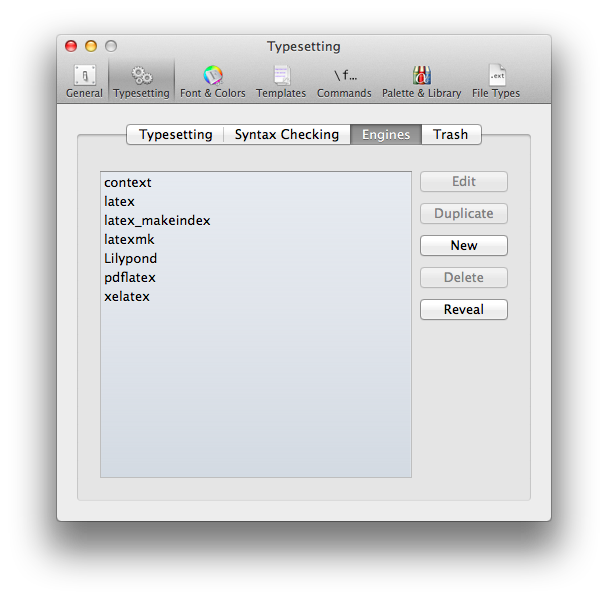
\includegraphics[width=0.8\textwidth]{reference/engines_pref_pane.png}
\caption{The preferences pane where you can edit and create engines.}
\label{fig:engines_pref_pane}
\end{figure}

\note{You can only edit engines which you create yourself. To edit one of the
built-in engines, you first need to duplicate it.}

Select one of the existing engines and click the ‘Duplicate’ button. You can
then go ahead and edit the duplicated engine script file.

On the ``Typesetting'' tab, you can set the default engine that is used for new
projects and documents. You can also give defaults values to some of the
configuration variables which are passed to the engines. Not all engines
support all configuration variables.


